\section{Frontend}
\subsection{Mock-Ups der Benutzerschnittstelle}
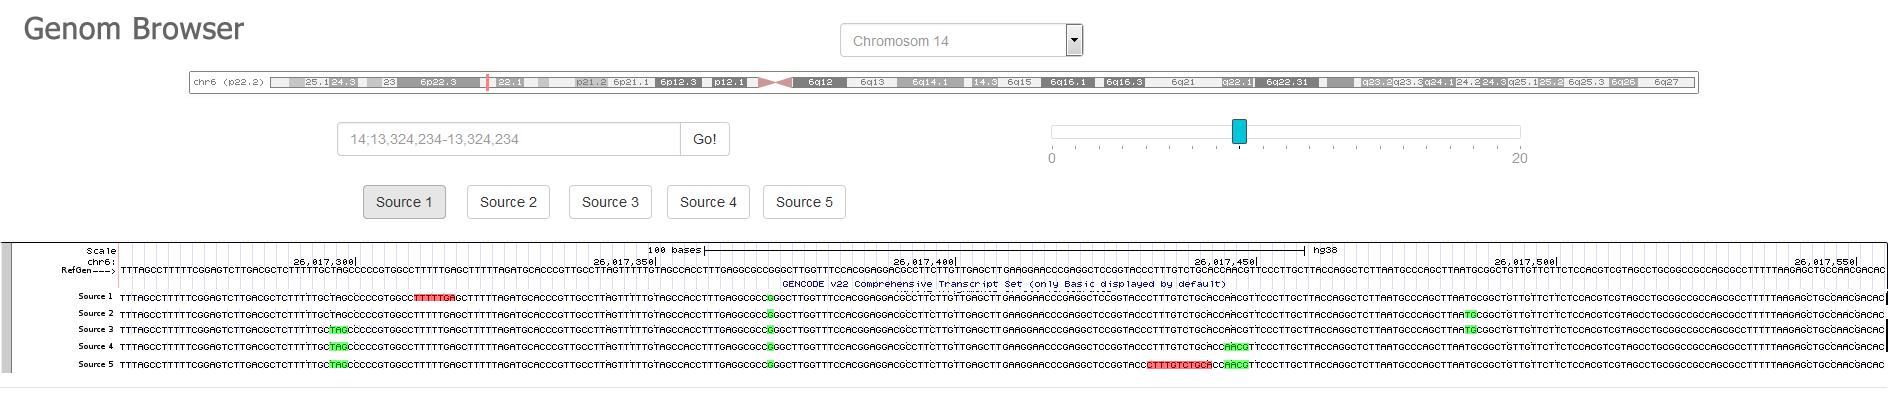
\includegraphics[width=\textwidth]{gui/gb_mockup_detail_view.png}
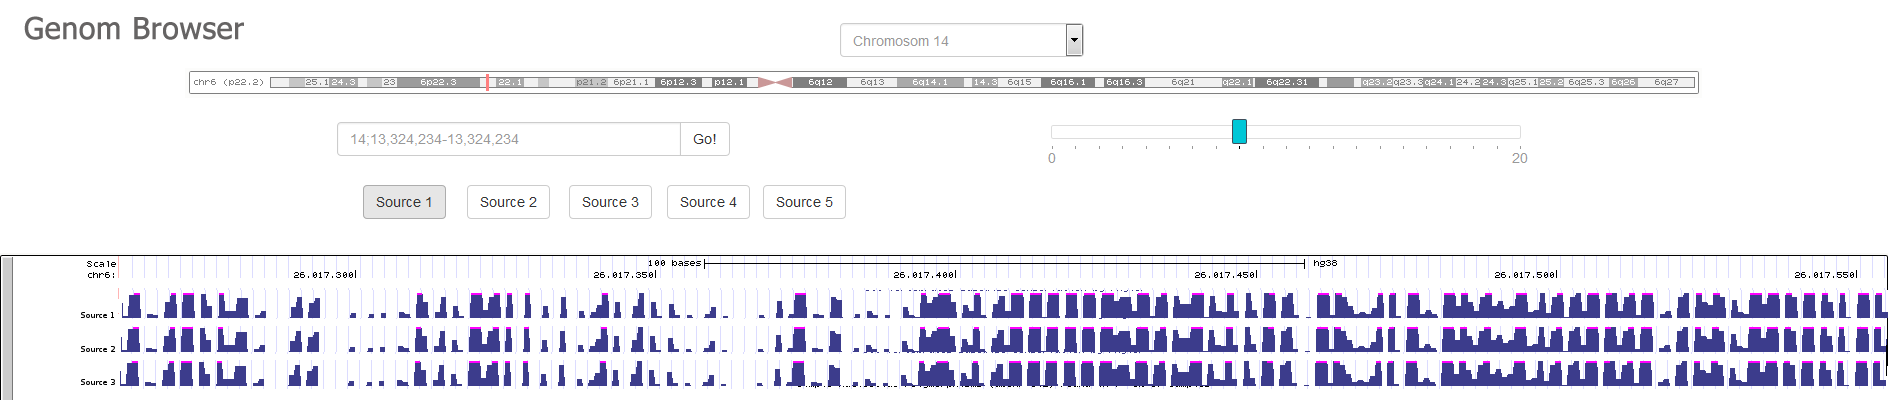
\includegraphics[width=\textwidth]{gui/gb_mockup_index_view.png}
\subsection{Klassen-Diagramm}
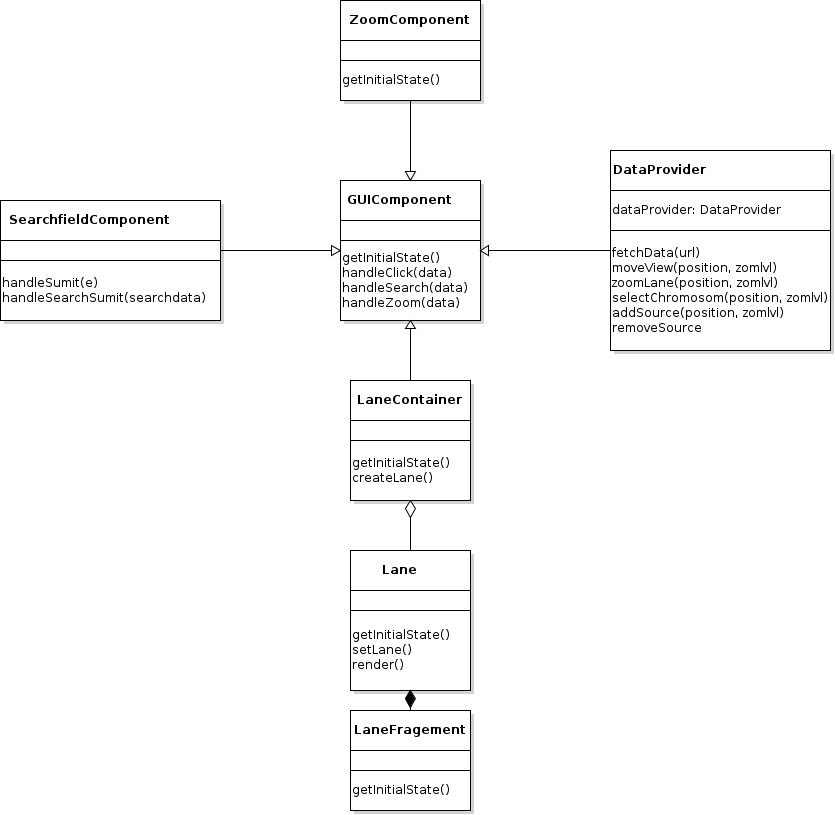
\includegraphics[width=\textwidth]{gui/gui-klassendiagramm.png}
\subsection{Sequenzdiagramm}
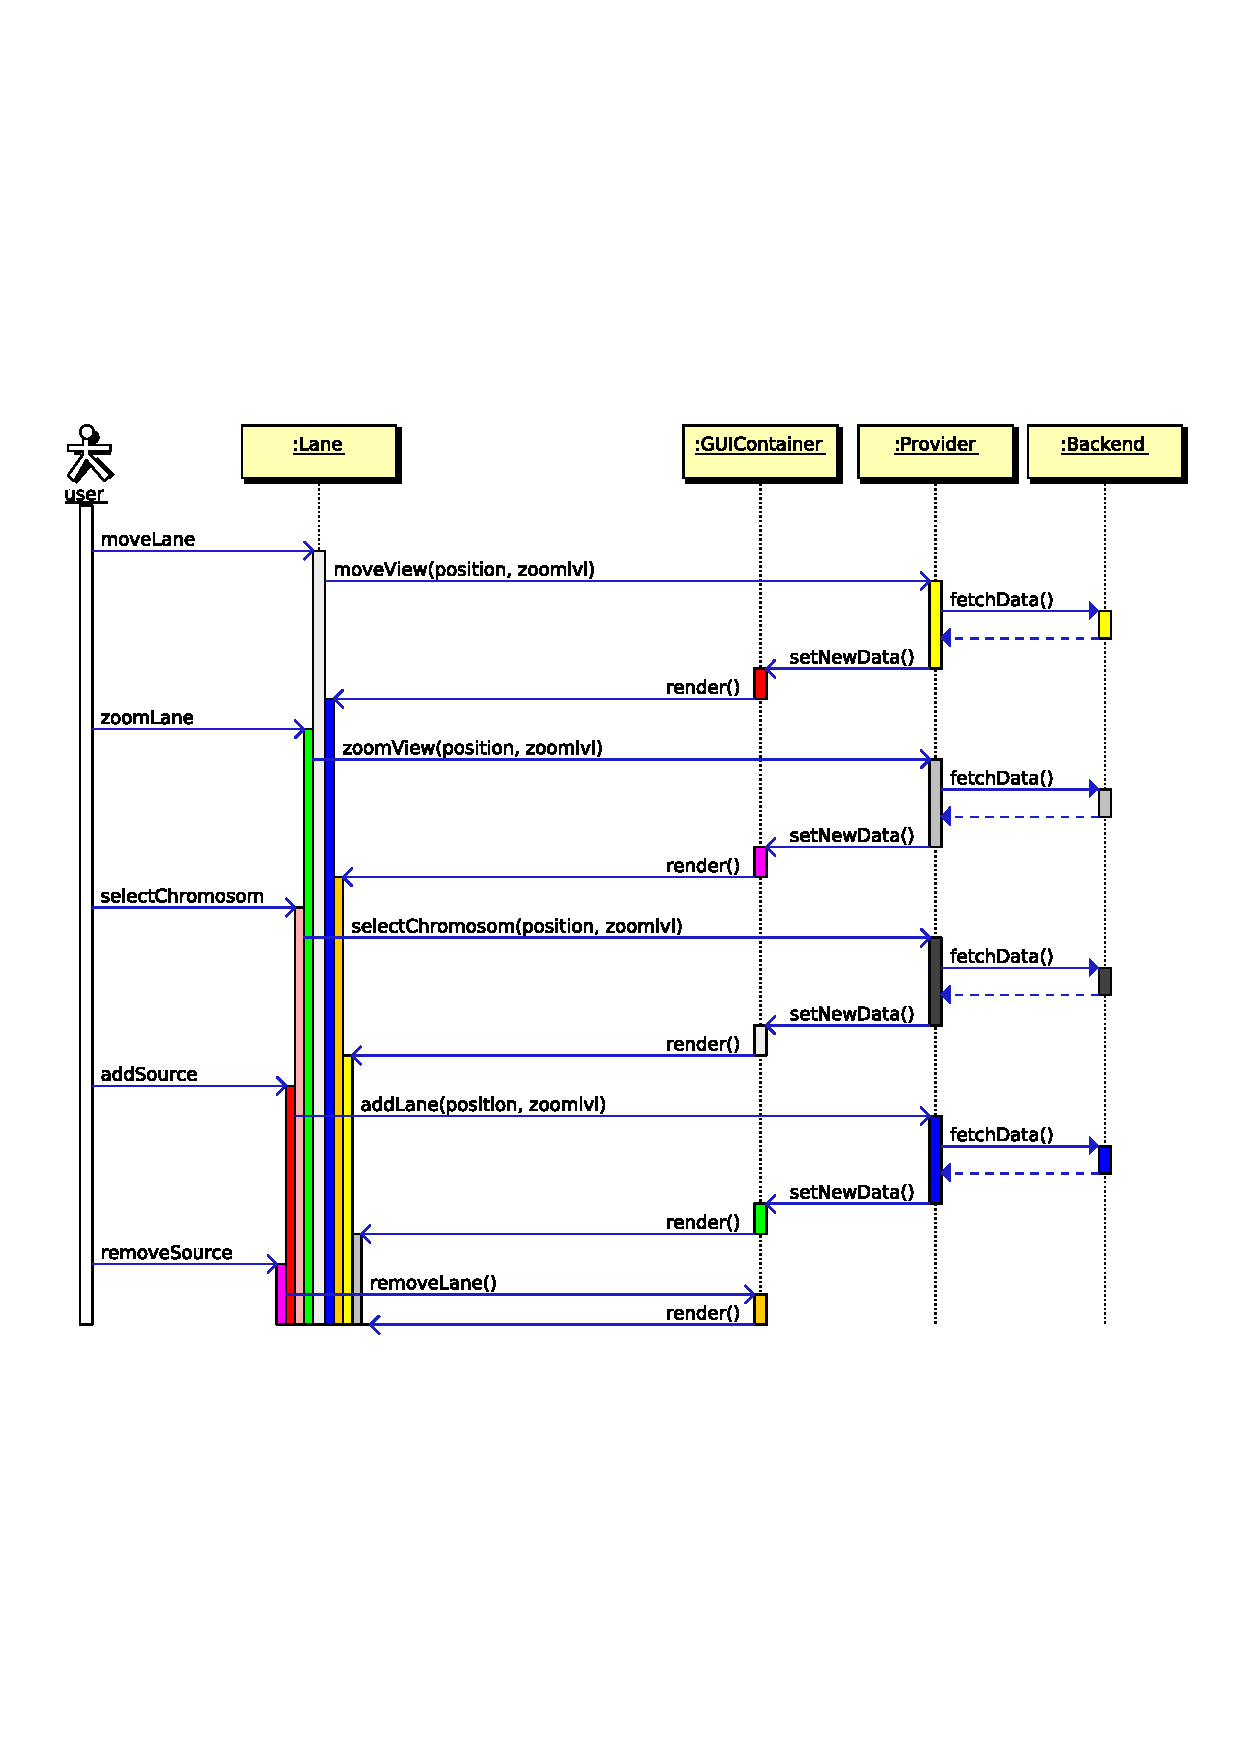
\includegraphics[width=\textwidth]{gui/GUI_Sequenzdiagramm.pdf}
\subsection{Use Cases}
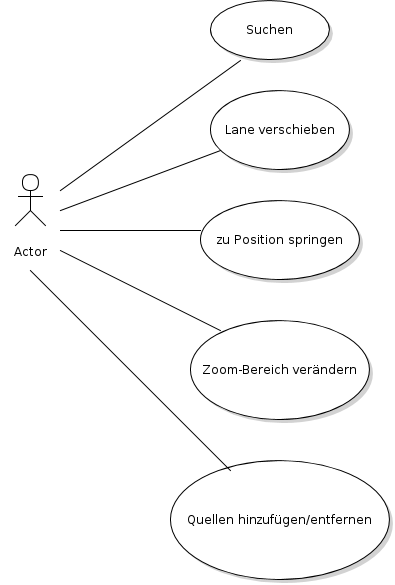
\includegraphics[width=\textwidth]{gui/gui-usecasediagramm.png}
\subsection{Unit-Tests}
\subsubsection{Suchfunktion}
\begin{enumerate}
	\item Wenn ich als Nutzer eine leere Suche starte, dann möchte ich eine entsprechende Fehlermeldung angezeigt bekommen.
	\item Wenn ich eine Suche mit falscher Eingabe starte, dann möchte ich eine entsprechende Fehlermeldung angezeigt bekommen.
	\item Wenn ich als Nutzer nach einem gültigen Intervall suche, dann wird automatisch die Zoomstufe auf dieses Intervall angepasst.
	\item Wenn ich als Nutzer nach einem vorhandenem Gene suche, dann wird automatisch die Zoomstufe auf dieses Intervall angepasst.
\end{enumerate}


\subsubsection{Quellen-Button}
\begin{enumerate}
	\item Wenn ich als Nutzer auf einen "Quellen"-Button drücke, dann wird mir die entsprechende Quelle zusätzlich zu den bereits dargestellten Quellen, angezeigt.
	\item Wenn ich als Nutzer auf den "Quellen"-Button einer bereits angezeigten Quelle drücke, wird die entsprechende Quelle nicht mehr angezeigt.
\end{enumerate}

\subsubsection{Quellen-Scroller}
\begin{enumerate}
	\item Als Nutzer kann ich mich über horizontales Scrolling synchron durch die Quellen bewegen.
\end{enumerate}

\subsubsection{Zoom-slider}
\begin{enumerate}
	\item Wenn ich die Zoomstufe über den Slider ändere, dann werden die Quellen entsprechend der eingestellten Stufe dargestellt.
	\item Wenn ich als Nutzer die feinste Zoomstufe einstelle, dann werden mir die Basenpaare angezeigt.
	\item Wenn ich als Nutzer eine andere Zoomstufe einstelle, dann werden mir aggregierten Daten angezeigt.
\end{enumerate}

\subsubsection{Chromosom-Auswahl}
\begin{enumerate}
	\item Als Nutzer kann ich über ein Dropdown aus einer Vorauswahl von Chromosomen auswählen.
	\item Wenn ich als Nutzer ein Chromosom auswähle, dann wird die Quellen-Anzeige automatisch entsprechend des ausgewählten Chromosoms aktualisiert.
	\item Wenn ich als Nutzer das bereits ausgewählte Chromosom erneut auswählen, dann passiert nichts.
\end{enumerate}

\subsubsection{Allgemein}
\begin{enumerate}
	\item Wenn ich als Nutzer auf eine Anfrage warten muss, wird mir dies durch einen Loading-Spinner signalisiert.	
\end{enumerate}
\newpage

%\section{Integrationstest}
%\subsection{Ablauf der Integrationstests}
